% questions.tex —— 1996 年·全国卷·理科 · 题目内容片段（无答案）
% 由 tools/generate_projects.py 依来源总账自 1996/1996_数学真题_全国理_试题.md 生成，勿手改（改源 MD 后重跑）


\begin{gktip}
固定来源：\texttt{普通高考/1996/1996全国理.pdf}，source ID 见来源校对记录，SHA-256 \texttt{cf9952ef5be41c7604605d651ada54a85217a4da09dfab19670a7a54cdc02bd4}。单页横向 A3，印刷页码 52。原页无答案、解析、分值或总分。发布者/版次及固定副本与原始出版物的关系未核。
\end{gktip}

\begin{question}
\gkti{1}已知全集 $I=\mathbb{N}$，集合 $A=\{x\mid x=2n,\ n\in\mathbb{N}\}$，$B=\{x\mid x=4n,\ n\in\mathbb{N}\}$，则\mbox{（　　）}。

（A）$I=A\cup B$　　（B）$I=\overline{A}\cup B$　　（C）$I=A\cup\overline{B}$　　（D）$I=\overline{A}\cup\overline{B}$

\Needspace{0.4\textheight}
\end{question}
\begin{question}
\gkti{2}当 $a>1$ 时，在同一坐标系中，函数 $y=a^{-x}$ 与 $y=\log_a x$ 的图象\mbox{（　　）}。
\nopagebreak[4]
\begin{center}% 固定来源PDF印刷页52第2题四组选项图象的矢量示意重绘。
% 单调性、截距及渐近线忠于原页；曲线斜率和坐标比例仅作示意。
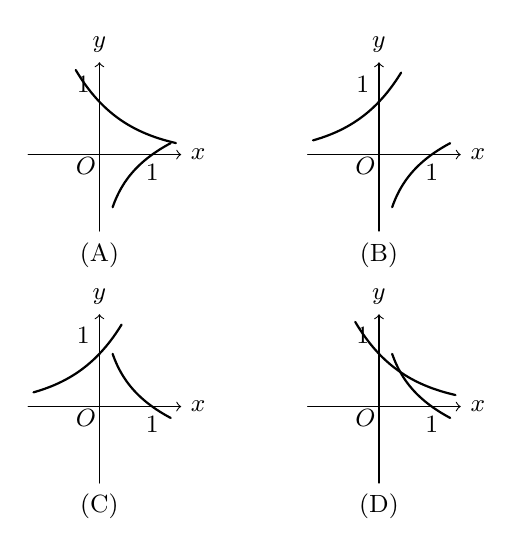
\begin{tikzpicture}[x=.67cm,y=.67cm,font=\small,line cap=round,line join=round]
  % (A) decreasing exponential and increasing logarithm.
  \begin{scope}
    \draw[->] (-1.35,0)--(1.55,0) node[right] {$x$};
    \draw[->] (0,-1.45)--(0,1.75) node[above] {$y$};
    \draw[thick,domain=-.45:1.45,samples=55,variable=\x] plot (\x,{exp(-1.05*\x)});
    \draw[thick,domain=.25:1.35,samples=55,variable=\x] plot (\x,{.72*ln(\x)});
    \node[below left,inner sep=1pt] at (0,0) {$O$};
    \node[above left] at (0,1) {$1$};
    \node[below] at (1,0) {$1$};
    \node at (0,-1.9) {(A)};
  \end{scope}

  % (B) increasing exponential and increasing logarithm.
  \begin{scope}[xshift=3.55cm]
    \draw[->] (-1.35,0)--(1.55,0) node[right] {$x$};
    \draw[->] (0,-1.45)--(0,1.75) node[above] {$y$};
    \draw[thick,domain=-1.25:.42,samples=55,variable=\x] plot (\x,{exp(1.05*\x)});
    \draw[thick,domain=.25:1.35,samples=55,variable=\x] plot (\x,{.72*ln(\x)});
    \node[below left,inner sep=1pt] at (0,0) {$O$};
    \node[above left] at (0,1) {$1$};
    \node[below] at (1,0) {$1$};
    \node at (0,-1.9) {(B)};
  \end{scope}

  % (C) increasing exponential and decreasing logarithm.
  \begin{scope}[yshift=-3.2cm]
    \draw[->] (-1.35,0)--(1.55,0) node[right] {$x$};
    \draw[->] (0,-1.45)--(0,1.75) node[above] {$y$};
    \draw[thick,domain=-1.25:.42,samples=55,variable=\x] plot (\x,{exp(1.05*\x)});
    \draw[thick,domain=.25:1.35,samples=55,variable=\x] plot (\x,{-.72*ln(\x)});
    \node[below left,inner sep=1pt] at (0,0) {$O$};
    \node[above left] at (0,1) {$1$};
    \node[below] at (1,0) {$1$};
    \node at (0,-1.9) {(C)};
  \end{scope}

  % (D) decreasing exponential and decreasing logarithm.
  \begin{scope}[xshift=3.55cm,yshift=-3.2cm]
    \draw[->] (-1.35,0)--(1.55,0) node[right] {$x$};
    \draw[->] (0,-1.45)--(0,1.75) node[above] {$y$};
    \draw[thick,domain=-.45:1.45,samples=55,variable=\x] plot (\x,{exp(-1.05*\x)});
    \draw[thick,domain=.25:1.35,samples=55,variable=\x] plot (\x,{-.72*ln(\x)});
    \node[below left,inner sep=1pt] at (0,0) {$O$};
    \node[above left] at (0,1) {$1$};
    \node[below] at (1,0) {$1$};
    \node at (0,-1.9) {(D)};
  \end{scope}
\end{tikzpicture}
\end{center}
\nopagebreak[4]
\end{question}
\begin{question}
\gkti{3}若 $\sin^2 x>\cos^2 x$，则 $x$ 的取值范围是\mbox{（　　）}。

（A）$\{x\mid 2k\pi-\frac{3\pi}{4}<x<2k\pi+\frac{\pi}{4},\ k\in\mathbb{Z}\}$

（B）$\{x\mid 2k\pi+\frac{\pi}{4}<x<2k\pi+\frac{5\pi}{4},\ k\in\mathbb{Z}\}$

（C）$\{x\mid k\pi-\frac{\pi}{4}<x<k\pi+\frac{\pi}{4},\ k\in\mathbb{Z}\}$

（D）$\{x\mid k\pi+\frac{\pi}{4}<x<k\pi+\frac{3\pi}{4},\ k\in\mathbb{Z}\}$

\end{question}
\begin{question}
\gkti{4}复数 $\dfrac{(2+2i)^4}{(1-\sqrt{3}i)^5}$ 等于\mbox{（　　）}。

（A）$1+\sqrt{3}i$　　（B）$-1+\sqrt{3}i$　　（C）$1-\sqrt{3}i$　　（D）$-1-\sqrt{3}i$

\end{question}
\begin{question}
\gkti{5}如果直线 $l,m$ 与平面 $\alpha,\beta,\gamma$ 满足：$l=\beta\cap\gamma$，$l\parallel\alpha$，$m\subset\alpha$，$m\perp\gamma$，那么必有\mbox{（　　）}。

（A）$\alpha\perp\gamma$ 且 $l\perp m$　　（B）$\alpha\perp\gamma$ 且 $m\parallel\beta$

（C）$m\parallel\beta$ 且 $l\perp m$　　（D）$\alpha\parallel\beta$ 且 $\alpha\perp\gamma$

\end{question}
\begin{question}
\gkti{6}当 $-\dfrac{\pi}{2}\le x\le\dfrac{\pi}{2}$，$f(x)=\sin x+\sqrt{3}\cos x$ 的\mbox{（　　）}。

（A）最大值是 $1$，最小值是 $-1$　　（B）最大值是 $1$，最小值是 $-\dfrac12$

（C）最大值是 $2$，最小值是 $-2$　　（D）最大值是 $2$，最小值是 $-1$

\end{question}
\begin{question}
\gkti{7}椭圆
\nopagebreak[4]
\[
\begin{cases}
x=3+3\cos\varphi,\\
y=-1+5\sin\varphi
\end{cases}
\]
的两个焦点坐标是\mbox{（　　）}。

（A）$(-3,5),(-3,-3)$　　（B）$(3,3),(3,-5)$

（C）$(1,1),(-7,1)$　　（D）$(7,-1),(-1,-1)$

\end{question}
\begin{question}
\gkti{8}若 $0<\alpha<\dfrac{\pi}{2}$，则
\nopagebreak[4]
\[
\arcsin\left[\cos\left(\frac{\pi}{2}+\alpha\right)\right]
+\arccos\left[\sin(\pi+\alpha)\right]
\]
等于\mbox{（　　）}。

（A）$\dfrac{\pi}{2}$　　（B）$-\dfrac{\pi}{2}$　　（C）$\dfrac{\pi}{2}-2\alpha$　　（D）$-\dfrac{\pi}{2}-2\alpha$

\end{question}
\begin{question}
\gkti{9}将边长为 $a$ 的正方形 $ABCD$ 沿对角线 $AC$ 折起，使得 $BD=a$，则三棱锥 $D-ABC$ 的体积为\mbox{（　　）}。

（A）$\dfrac{a^3}{6}$　　（B）$\dfrac{a^3}{12}$　　（C）$\dfrac{\sqrt{3}}{12}a^3$　　（D）$\dfrac{\sqrt{2}}{12}a^3$

\end{question}
\begin{question}
\gkti{10}等比数列 $\{a_n\}$ 的首项 $a_1=-1$，前 $n$ 项和为 $S_n$，若 $\dfrac{S_{10}}{S_5}=\dfrac{31}{32}$，则 $\displaystyle\lim_{n\to\infty}S_n$ 等于\mbox{（　　）}。

（A）$\dfrac23$　　（B）$-\dfrac23$　　（C）$2$　　（D）$-2$

\end{question}
\begin{question}
\gkti{11}椭圆的极坐标方程为 $\rho=\dfrac{3}{2-\cos\theta}$，则它在短轴上的两个顶点的极坐标是\mbox{（　　）}。

（A）$(3,0),(1,\pi)$

（B）$\left(\sqrt{3},\dfrac{\pi}{2}\right),\left(\sqrt{3},\dfrac{3\pi}{2}\right)$

（C）$\left(2,\dfrac{\pi}{3}\right),\left(2,\dfrac{5\pi}{3}\right)$

（D）$\left(\sqrt{7},\arctan\dfrac{\sqrt{3}}{2}\right),\left(\sqrt{7},2\pi-\arctan\dfrac{\sqrt{3}}{2}\right)$

\end{question}
\begin{question}
\gkti{12}等差数列 $\{a_n\}$ 的前 $m$ 项和为 $30$，前 $2m$ 项和为 $100$，则它的前 $3m$ 项和为\mbox{（　　）}。

（A）130　　（B）170　　（C）210　　（D）260

\end{question}
\begin{question}
\gkti{13}设双曲线 $\dfrac{x^2}{a^2}-\dfrac{y^2}{b^2}=1\ (0<a<b)$ 的半焦距为 $c$，直线 $l$ 过 $(a,0),(0,b)$ 两点，已知原点到直线 $l$ 的距离为 $\dfrac{\sqrt{3}}{4}c$，则双曲线的离心率为\mbox{（　　）}。

（A）$2$　　（B）$\sqrt{3}$　　（C）$\sqrt{2}$　　（D）$\dfrac{2\sqrt{3}}{3}$

\end{question}
\begin{question}
\gkti{14}母线长为 $1$ 的圆锥体积最大时，其侧面展开图圆心角 $\varphi$ 等于\mbox{（　　）}。

（A）$\dfrac{2\sqrt{2}}{3}\pi$　　（B）$\dfrac{2\sqrt{3}}{3}\pi$　　（C）$\sqrt{2}\pi$　　（D）$\dfrac{2\sqrt{6}}{3}\pi$

\end{question}
\begin{question}
\gkti{15}设 $f(x)$ 是 $(-\infty,+\infty)$ 上的奇函数，$f(x+2)=-f(x)$，当 $0\le x\le1$ 时，$f(x)=x$，则 $f(7.5)$ 等于\mbox{（　　）}。

（A）$0.5$　　（B）$-0.5$　　（C）$1.5$　　（D）$-1.5$

\end{question}
\begin{question}
\gkti{16}已知圆 $x^2+y^2-6x-7=0$ 与抛物线 $y^2=2px\ (p>0)$ 的准线相切，则 $p=\underline{\qquad\qquad}$。

\end{question}
\begin{question}
\gkti{17}正六边形的中心和顶点共 $7$ 个点，以其中 $3$ 个点为顶点的三角形共有$\underline{\qquad\qquad}$个。（用数字作答）

\end{question}
\begin{question}
\gkti{18}$\tan20^\circ+\tan40^\circ+\sqrt{3}\tan20^\circ\tan40^\circ$ 的值是$\underline{\qquad\qquad}$。

\Needspace{0.4\textheight}
\end{question}
\begin{question}
\gkti{19}如图，正方形 $ABCD$ 所在平面与正方形 $ABEF$ 所在平面成 $60^\circ$ 的二面角，则异面直线 $AD$ 与 $BF$ 所成角的余弦值是$\underline{\qquad\qquad}$。
\nopagebreak[4]
\begin{center}% 固定来源PDF印刷页52第19题两个正方形的示意重绘。
% 顶点关联及共边忠于原图，投影边长不代表空间角度的精确比例。
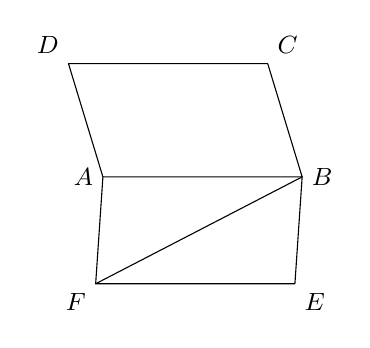
\begin{tikzpicture}[scale=1.15,line join=round,line cap=round,
  every node/.style={font=\small}]
\coordinate (A) at (0,0);
\coordinate (B) at (2.2,0);
\coordinate (D) at (-.38,1.25);
\coordinate (C) at (1.82,1.25);
\coordinate (F) at (-.08,-1.18);
\coordinate (E) at (2.12,-1.18);
\draw (A)--(D)--(C)--(B)--cycle;
\draw (A)--(F)--(E)--(B);
\draw (B)--(F);
\node[left] at (A) {$A$};
\node[right] at (B) {$B$};
\node[above left] at (D) {$D$};
\node[above right] at (C) {$C$};
\node[below left] at (F) {$F$};
\node[below right] at (E) {$E$};
\end{tikzpicture}
\end{center}
\nopagebreak[4]
\end{question}
\begin{question}
\gkti{20}解不等式：$\log_a\left(1-\dfrac{1}{x}\right)>1$。

\end{question}
\begin{question}
\gkti{21}已知 $\triangle ABC$ 的三个内角 $A,B,C$ 满足：$A+C=2B$，
\nopagebreak[4]
\[
\dfrac{1}{\cos A}+\dfrac{1}{\cos C}=-\dfrac{\sqrt{2}}{\cos B},
\]
求 $\cos\dfrac{A-C}{2}$ 的值。

\Needspace{0.4\textheight}
\end{question}
\begin{question}
\gkti{22}如图，在正三棱柱 $ABC-A_1B_1C_1$ 中，$E\in BB_1$，截面 $A_1EC\perp\text{\text{侧面} }AC_1$。

（1） 求证：$BE=EB_1$；

（2） 若 $AA_1=A_1B_1$，求平面 $A_1EC$ 与平面 $A_1B_1C_1$ 所成二面角（锐角）的度数。
\nopagebreak[4]
\begin{center}% 固定来源PDF印刷页52第22题正三棱柱及截面的示意重绘。
% E位于BB1中点；透视尺寸仅用于表示点线关系，不作为度量条件。
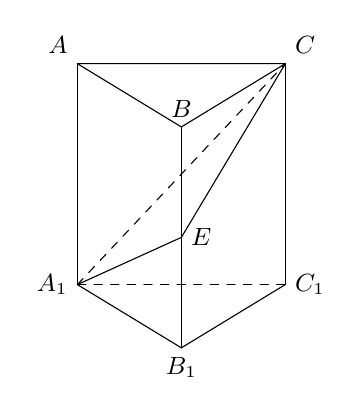
\begin{tikzpicture}[scale=1.1,line join=round,line cap=round,
  every node/.style={font=\small}]
\coordinate (A) at (0,2.55);
\coordinate (B) at (1.2,1.82);
\coordinate (C) at (2.4,2.55);
\coordinate (Aone) at (0,0);
\coordinate (Bone) at (1.2,-.73);
\coordinate (Cone) at (2.4,0);
\coordinate (E) at (1.2,.545);
% Two triangular bases and the connecting edges.
\draw (A)--(B)--(C)--cycle;
\draw (A)--(Aone) (B)--(Bone) (C)--(Cone);
\draw (Aone)--(Bone)--(Cone);
\draw[dashed] (Aone)--(Cone);
% Cross-section A1EC; A1C and the hidden base edge are dashed in the source.
\draw (Aone)--(E)--(C);
\draw[dashed] (Aone)--(C);
\node[above left] at (A) {$A$};
\node[above] at (B) {$B$};
\node[above right] at (C) {$C$};
\node[left] at (Aone) {$A_1$};
\node[below] at (Bone) {$B_1$};
\node[right] at (Cone) {$C_1$};
\node[right] at (E) {$E$};
\end{tikzpicture}
\end{center}
\nopagebreak[4]
\end{question}
\begin{question}
\gkti{23}某地现有耕地 $10000$ 公顷，规划 $10$ 年后粮食单产比现在增加 $22\%$，人均粮食占有量比现在提高 $10\%$。如果人口年增长率为 $1\%$，那么耕地平均每年至多能减少多少公顷（精确到 $1$ 公顷）？

（粮食单产$=\dfrac{\text{\text{总产量}}}{\text{\text{耕地面积}}}$，人均粮食占有量$=\dfrac{\text{\text{总产量}}}{\text{\text{总人口数}}}$。）

\end{question}
\begin{question}
\gkti{24}已知 $l_1,l_2$ 是过点 $P(-\sqrt{2},0)$ 的两条互相垂直的直线，且 $l_1,l_2$ 与双曲线 $y^2-x^2=1$ 各有两个交点，分别为 $A_1,B_1$ 和 $A_2,B_2$。

（1） 求 $l_1$ 的斜率 $k_1$ 的取值范围；

（2） 若 $\left|A_1B_1\right|=\sqrt{5}\left|A_2B_2\right|$，$l_1$，求 $l_1,l_2$ 的方程。

\end{question}
\begin{question}
\gkti{25}已知 $a,b,c$ 是实数，函数 $f(x)=ax^2+bx+c$，$g(x)=ax+b$，当 $-1\le x\le1$ 时，$|f(x)|\le1$。

（1） 证明：$|c|\le1$；

（2） 证明：当 $-1\le x\le1$ 时，$|g(x)|\le2$；

（3） 设 $a>0$，当 $-1\le x\le1$ 时，$g(x)$ 的最大值为 $2$，求 $f(x)$。

\end{question}